\chapter{Systementwurf}\label{chp:systementwurf}


%#######################################################################################
%#######################################################################################
\section{Variantenmanagement und Parameter}
\paragraph{}

Die Lösung zum Speichern und Darstellen der Parameterwerte abhängig der aktiven Variante wurde folgendermaßen programmiert.\\

\begin{figure}[h!]
  \begin{center}
    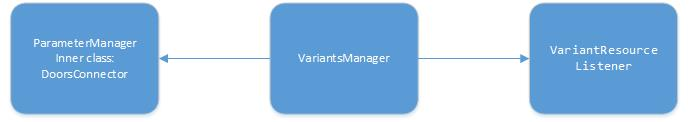
\includegraphics[scale=0.7]{5_1_klassenuebersicht.jpg}
  		  \caption{Darstellung der Klassen}
     \label{ttn.verbindung.klassen.loesung}
  \end{center}
\end{figure}



%#######################################################################################
\subsection{ResourceSetListener}
Das auslösendes Element ist, dass der Benutzer eine Anforderung mit einen Baumelement verknüpft. Um dieses Geschehen abzufragen wurde ein \textit{Listener} programmiert, der das Interface \textit{ResourceSetListener}\footnote{http://download.eclipse.org/modeling/emf/transaction/javadoc/1.0.3/org/eclipse/emf/transaction/ResourceSetListener.html} implementiert. Die Aufgabe des \textit{ResourceSetListener} ist, dem Benutzer zu benachrichtigen, wenn sich eine Ressource ändert. Der \textit{Listener}  \glqq hört\grqq~ auf die reinkommenden Nachrichten (\textit{ResourceSetChangeEvent}) und wertet den Inhalt dieses Events aus.\\

Als Inhalt der Nachricht wird folgendes empfangen: 

\begin{itemize}
\item \textbf{Event: }ResourceSetChangeEvent, heißt die Ressourcen des Objektes haben sich geändert
\item \textbf{Notifier: } welches Objekt schickt die Nachricht
\item \textbf{Notification: }Beschreibung von der Änderung im \textit{Notifier}
\item \textbf{OldValue: } alter Wert, wenn nicht vorhanden \textit{null}
\item \textbf{NewValue: } neuer Wert, beim löschen von Werten \textit{null}
\end{itemize}

Hier wird als erstes der \textit{Notifier} abgefragt um zu unterscheiden, ob die Nachricht für uns relevant ist. Ist der \textit{Notifier} eine Instanz eines Baumelementes, so wurde eine Anforderung zum ersten mal an das Baumelement verknüpft. \\

Lautet der \textit{Notifier} Instanz von \textit{RequirementTag} so wurde eine Anforderung von einem Baumelement gelöscht oder es wurde eine neue Anforderung an einen Baumelement hinzugefügt, wo schon Anforderung verknüpft waren. Für alle drei Fälle muss der \textit{Listener} wissen:

\begin{itemize}
\item An welches Element wurde das Event ausgelöst?
\item Welche Anforderung wurde hinzugefügt oder gelöscht?
\end{itemize}

Dafür wird aus dem \textit{Notifier} mit der Methode \texttt{getID()} die Identifikationsnummer des zuständiges Baumelement abgefragt. Weiterhin steht im \textit{Notifier} auch die Kennung der Anforderung (diese wurde in DOORS vergeben). Diese beide Informationen werden gespeichert und an den \textit{VariantsManager} weiter gegeben. Diese Informationen sind für der \textit{ParameterManager} nötig, damit er aus der Anforderung die Parameter lesen kann und mit das richtige Baumelement verknüpfen kann.\\




%#######################################################################################
\subsection{VariantsManager}\label{sub.VariantsManager}
Die Hauptaufgabe des \textit{VariantsManager} ist die Varianten zu regeln. Hier werden Baumelemente zu  Varianten hinzugefügt und gelöscht. Dabei muss das Klassifikationsbaum neu gezeichnet werden. Diese Klasse kümmert sich auch, um die Umschaltung zwischen Varianten in der Variantenansicht (siehe Abbildung \ref{ttn.generic}). Der \textit{VariantsManager} setzt die Baumelement-ID und die Anforderungskennung in der Klasse \textit{ParameterManager}. Die Klasse dient als Schnittstelle zwischen der \textit{Listener} und die Klasse \textit{ParameterManager}\\

Der \textit{VariantsManager} fragt den \textit{Editor} (beinhaltet das Klassifikationsbaum) nach das benötigte Baumelement über die von \textit{Listener} übergebene Identifikationsnummer. Das Baumelement wird dann in das \textit{ParameterManager} gespeichert. Die Anforderungskennung wird auch im Objekt von \textit{ParameterManager} gespeichert.\\



Requirement IndieModul im connection eigenschaften!!\\


%#######################################################################################
\subsection{Parameter-\textit{Tag}}\label{sub.ParameterTag}
\subsubsection{ParameterTag}
Das Interface dient als Schnittstelle für den Zugriff auf das Inhalt von ParameterTagImpl. Das Interface erweitert \textit{Tag}. Das \textit{Tag} Interface ist ein in TESTONA allgemein implementiertes Modell, welches auf ein Interface und eine implementierende Klasse basiert. Für jedes \textit{Tag} (RequirementTag, VariantTag, etc.) gibt es ein eine Klasse. In das Interface wird immer das Tagtyp definiert um \textit{Tags} voneinander unterscheiden zu können.

\begin{lstlisting}[caption={ParameterTag Interface}, captionpos=b]
public static final String TAGTYPE = "ParameterTag";
\end{lstlisting}

Das Tagmodell wird benutzt um in TESTONA überall ähnliche Objekt zu haben, die verschiedene Funktionen erfühlen, aber die gleiche Richtlinie folgen

\subsubsection{ParameterTagImpl}
Die Klasse \textit{ParameterTagImpl} erweitert die Klasse \textit{TagImpl} und implementiert \textit{ParameterTag}. In dieser Klasse werden die Vorteile von das Tagmodell deutlicher. Die Klasse \textit{TagImpl} definiert sehr nützliche Methoden und Eigenschaften die in \textit{ParameterTagImpl} angewendet werden.\\

Jedes \textit{Tag} hat als Eigenschaft einen Namen. In diese Klasse entspricht der Name, ein Parametername der aus der Parametertabelle gelesen wurde. Weiterhin ist über \textit{ID} eine eindeutige Identifikationsnummer definiert, um \textit{Tags} des gleichen Typs voneinander zu unterscheiden.\\

Der Inhalt von das \textit{Tag} ist durch ein \textit{EcoreEMap<String, String>} definiert. Das erste String ist ein Schlüsselwert und das zweite String das Wert. Im diesem Fall ist der Schlüssel der Name einer Variante, und der Wert ist der Parameterwert des Parameters in dieser Variante.  Anhand der Methode \textit{getContent()} kann der Inhalt eines \textit{Tags} aufgerufen werden und mit der Methode \textit{addEntry()} werden Inhalte hinzugefügt. Das Gegenteil kann man mit der Methode \textit{deleteEntry()} erreichen. Wie die Methoden genauer angewendet werden, wird im Listing \ref{lst:CreateParamTag} gezeigt.



serialize und unserialize\\


%#######################################################################################
\subsection{ParameterManager}\label{sub.ParameterManager}

%\begin{figure}[h!]
%  \begin{center}
%    \includegraphics[scale=0.7]{.jpg}
%  		  \caption{Darstellung der Klasse ParameterManager in UML}
%     \label{ttn.ParameterMananger}
%  \end{center}
%\end{figure}

Die Klasse \textit{ParameterManager} beinhaltet eine private innere Klasse \textit{DoorsConnector}(siehe \ref{sub.DoorsConn}), diese kümmert sich um den Verbindungsaufbau mit DOORS.\\ Weiterhin baut die Klasse die vom \textit{Listener} weitergegeben Daten (Baumelement und Anforderungskennung) auf.\\



Anforderung eines Baumelementes beinhaltet Modul und Interface. wichtig für nächstes Kapitel\\

IndieModul : interId: doors, connId: localhost;36677, moduleId: /Simple Belt Warner 2/Simple Belt Warner Spec, moduleNbr: 0, id: doors,localhost;36677,/Simple Belt Warner 2/Simple Belt Warner Spec)\\


\begin{lstlisting}[caption={Erstellung der ParameterTag}, captionpos=b,label={lst:CreateParamTag}]
ParameterTag tempTag = new ParameterTagImpl();
		
for(int i = 0; i < attributesList.size(); i++){
	
	//An der nullte Stelle steht immer der Parametername
	if(i == 0) {
		tempTag.setName(req.getValue(attributesList.get(0)).getValueAsString());
	} else {
		//entferne " Value" vom Variantenamen 
		tempTag.addEntry(sAttrList.get(i).substring(0, sAttrList.get(i).lastIndexOf("Value")-1),
				req.getValue(attributesList.get(i)).getValueAsString());
	}
}
paramTagList.add(tempTag);
\end{lstlisting}


%#######################################################################################
\subsection{AddParameterTagCommand}\label{sub.Command}



%#######################################################################################
\subsection{Die DOORS Verbindng}\label{sub.DoorsConn}
\subsubsection{DoorsConnector}
%\begin{figure}[h!]
%  \begin{center}
%    \includegraphics[scale=0.7]{.jpg}
%  		  \caption{Darstellung der innere Klasse DoorsConnector in UML}
%     \label{ttn.DoorsConnetor}
%  \end{center}
%\end{figure}

Die private innere Klasse \textit{DoorsConnector} baut die Verbindung zwischen den TESTONA und DOORS auf. Sie implementiert das Interface \textit{IConnectionListener}, dass ein \textit{Listener} für die Verbindung - Events umfasst. Für das Laden von Dateien aus DOORS benötigt die Klasse noch ein \textit{Listener} (IDataListener) und ein \textit{Adapter}(IReqLoadAdapter) \\

Als erstes wird von der Klasse \textit{ParameterManager} die Methode \textit{connectToDoors()} aufgerufen. Diese baut die Verbindung auf, indem gespeicherte Verbindungsdaten aufgerufen werden. Wie bereits in Kapitel \ref{sub.ParameterManager} erwähnt, beinhaltet eine Anforderung die Informationen wo die Anforderung gespeichert ist (welches DOORS Modul und über welches Interface das Modul zu erreichen ist). Für den Verbindungsaufbau werden folgende Objekte benötigt:

\begin{itemize}
\item \textbf{DataInterface: }Über diese Klasse erfolgt die Datenanfrage an DOORS. Die Verbindung wird aufgebaut sowie getrennt. Es werden als erstes die Ordner geladen, danach einzelne Projekte und die nötige Module. Es können verschiedene Darstellungen der Module auch geladen werden (diese müssen in DOORS definiert sein). Hier werden auch direkt einzelne Anforderungen angefragt. Relevant für diese Arbeit ist, dass hiermit das Modul Parametertabelle in DOORS geladen wird.

\item \textbf{PreferenceManagment: } Hier werden die in TESTONA gespeicherte Verbindungsdaten behandelt. Es können Microsoft Access Verbindungensdaten gespeichert werden, aber wir werde nur DOORS betrachten.

\item \textbf{Connector: }beschreibt eine einzelne Verbindung, hat ein \textit{DataIterface}- und \textit{PreferenceManagmentobjekt}

\item \textbf{ConnectionManager: }Singleton. Die Klasse handelt aktive und offene Verbindungen. Hier werden die \textit{ConnectionListeners} und das \textit{DataInterface} für den richtigen \textit{Connector} geregelt.

\end{itemize}


Um die Verbindung mit DOORS aufzubauen muss als erstes die Instanz des \textit{ConnecionManagers} lokal referenziert werden (weil es ein \textit{Singleton} ist, darf kein neues Objekt erzeugt werden). Wenn die Instanz des \textit{ConnectionManagers} geladen ist, kann jetzt der \texttt{connector} aus dem \textit{ConnectionManager} aufgerufen werden.

\begin{lstlisting}[caption={Verbindungsaufbau}, captionpos=b]
try {
	connector = ConnectorManager.getInstance()
				.getConnector(im.getInterId());
	dataInterface = conManager.getNewDataInterface(connector, this);
} catch (ExtensionException e) {
	e.printStackTrace();
}
\end{lstlisting}

 Um dem richtigen \texttt{connector} aufzurufen muss aus das \textit{IndieModul} (\texttt{im.getInterId()}, siehe Kapitel \ref{sub.VariantsManager}) die Interfacekennung als Übergabeparameter angegeben werden. Als nächstes kann über den \textit{ConnectionManager} eines neues \textit{DataInterface} erzeugt werden, wo der \texttt{connector} und das aktuelle Objekt (\textit{DoorsConnector}) übergeben werden.\\
 
Aus den in TESTONA gespeicherte Verbindungspräferenzen werden die Verbindungsparameter für DOORS geladen. An dieser Stelle braucht das \textit{DataInterface} die nötige \textit{Listeners} bevor die Verbindung aufgebaut wird. Durch die Methode \textit{addListener(listener)} wird das \textit{RequirementDataListener} und das \textit{IConnectionListener} (von \textit{DoorsConnetor} implementiert) gesetzt. Mit dem Aufruf der Methode \textit{connecteInterface(Verbindungsparameter)} wird das \textit{DataInterface} an DOORS verbunden.\\

Der Grund warum ein \textit{IConnectionListener} implementiert wird, lautet dass der Verbindungsaufbau in einem neuen Thread stattfindet. Das \textit{DoorsConnetor} Objekt wird über das \textit{IConnectionListener} benachrichtigt ob die Verbindung stattgefunden hat. Die Methode\texttt{interfaceConnected} (aus dem \textit{IConnectionListener}) wird aufgerufen, wenn die Verbindung erfolgreich entstanden ist.

\begin{lstlisting}[caption={Verbindungsaufbau was erfolgreich}, captionpos=b]
@Override
public void interfaceConnected() {
	connected = true;
	reqDataListener.setListener(reqLoadListener);
	dataInterface.loadModule(PARAM_PATH, this, false);
}
\end{lstlisting}

Der gesetzte \textit{RequirementDataListener} benötigt ein \textit{RequirementLoadListener}, dass eine rückmeldung gibt, wenn die Zeilen aus einer Tabelle fertig geladen worden sind. Die Tabelle wird anhand der Methode \texttt{loadModule} wird ein DOORS Modul (Tabelle) geladen. Welches Modul geladen wird, spezifiziert der Parameter \texttt{PARAM\_PATH}. Es gibt an wo sich das Modul in der DOORS Datenbank befindet. Der \textit{RequirementDataListener} erhält die Nachricht, dass ein Modul geladen worden ist. Weiter dazu wird im Kapitel \ref{sub.RequirementDataListener} erläutert.\\


Es wird angenommen, wenn der Benutzer die Parameterersetzung für ein Parameter wahrnimmt, dass er es für weitere Parameter wahrnehmen wird. Da die Datenmenge von einer Parametertabelle relativ gering ist, wurde hier, bezüglich der offene Frage bei dem Lösungsansatz (siehe Kapitel \ref{sec.parameterspeicherung}), die Parametertabelle komplett importiert. 
Ein weiterer Grund lautet, dass nicht für jeder Parameter erneut eine DOORS Verbindgun enstehen muss. So wird die Rechen- und Reaktionszeit von TESTONA so weit es geht gering gehalten. Die Parametertabelle wird erst bei der Verknüpfung von einer Anforderung mit einem Baumelement importiert und nicht beim Import der Anforderungen. 

Wenn die Parametertabelle komplett geladen wurde, ermöglicht die Methode \textit{closeConnection} die Verbindung mit DOORS zu beenden und das \textit{DataInterface} zu schließen.





\subsubsection{RequirementDataListener}\label{sub.RequirementDataListener}

Ist ein Event-Listener, dass auf die Rückmeldung vom Laden eines Moduls wartet. Relevant ist die Methode \texttt{onModuleLoad} die die Zeilen aus der Tabelle liest und speichert.\\

\begin{lstlisting}[caption={Laden der Parametertabelle nach Zeilen}, captionpos=b]
@Override
public void onModuleLoad(Module module, Object family, boolean reload){

	BasicRequirement baseReq;
	saveAttributesNames(module);
				
	for (String reqId : module.getRequirementIds()) {

		baseReq = dataInterface.getRequirement(module, reqId,
				reqLoadListener);

		if (baseReq.checkStatus(BasicRequirement.STATUS_LOADED)){
			paramReqList.add((Requirement) baseReq);
			fillParamTagList((Requirement) baseReq);
		}
	}
	dataInterface.flush(reqLoadListener);
}
\end{lstlisting}

Zu beachten ist, dass in DOORS jede Zeile in einer Tabelle als eine Anforderung (eng. Requirement) gesehen wird. Daher heißen Variablen und Methoden oft \glqq Requirement\grqq~ oder Abkürzung des Wortes (req). Die Methode \texttt{saveAttributesNames} speichert die im geladenes Modul vorhandenen Attribute. Im diesem Fall (treu zum Beispiel mit dem Auto) sind es:

\begin{itemize}\itemsep1pt
\item Paramenter Name
\item Default Value
\item Cabrio Value
\item Kombi Value
\item Limo Value
\end{itemize}

Diese Attribute repräsentieren die Varianten und ein Standardwert, sowie der Name des jeweiligen Parameter. In der Schleife werden alle Zeilen im Modul iteriert und geladen. Wenn die Zeile (\texttt{baseReq}) vollständig geladen wurde, wird diese in der globalen Liste \texttt{paramReqList} als ein \texttt{Requirement} Objekt gespeichert. Die Methode \texttt{fillParamTagList} erzeugt die \textit{ParameterTags} und wurde in Kapitel \ref{sub.ParameterManager} erläutert.\\

Wenn eine Zeile nicht vollständig geladen werden konnte, gibt es das \textit{RequirementLoadListener}, dass sich um das vollständige laden der Zeilen kümmert. Das \textit{RequirementLoadListener} wird in dieser Klasse instantiiert und von der \textit{DoorsConnetor} Klasse gesetzt. Weiter dazu im nächsten Kapitel.


\subsubsection{RequirementLoadListener}\label{sub.RequirementLoadListener}
Der \textit{RequirementLoadListener} reagiert wenn eine Zeile nicht völlstandigt geladen worden ist, und wartet bis diese geladen wird. Die Methode \texttt{onLoad} bekommt als Eingabeparameter eine Liste der nicht geladenen Zeilen.

\begin{lstlisting}[caption={Nachladen der Parametertabelle nach Zeilen}, captionpos=b]
public void onLoad(List<BasicRequirement> requirements) {

	for (BasicRequirement baseReq : requirements) {
		paramReqList.add((Requirement) baseReq);
		fillParamTagList((Requirement) baseReq);
		
	}
}
\end{lstlisting}

Diese Liste wird iteriert und wie in Kapitel \ref{sub.RequirementDataListener} in der globalen Liste \texttt{paramReqList} als ein \texttt{Requirement} Objekt gespeichert.\\

Weiterhin meldet diese Klasse wenn alle Zeilen aus das DOORS Modul geladen wurden. Das wartenden Dialogfenster aus \ref{sub.ParameterManager} wird benachrichtigt, dass es geschlossen werden kann. Die Benutzeroberfläche von TESTONA ist somit wieder für den Benutzer erreichbar.


%#######################################################################################
%#######################################################################################
\newpage
\section{Testfallgenerierung und Optimierung}
\paragraph{}
Erläuterung der Lösungen zu 4.3